\section{Design}
\label{sec:design}

The empirical study establishes one overarching requirement: connect
AI agent intent and project or task context to deterministic OS-level
enforcement.
Achieving this raises three design challenges.

\textbf{C1: Agent-authorable OS-level policy} (\S\ref{sec:dsl}).
74\% of system-observable directives require project or task context that
only the agent possesses, so the agent must author its own enforcement
rules. Yet OS-level enforcement demands concrete, deterministic
predicates. The policy language must be simple enough for an LLM to
generate correctly, yet compile to efficient kernel-level matching.

\textbf{C2: Cross-event state at syscall speed} (\S\ref{sec:ifc}).
81\% of repositories require policies that span multiple
operations: ``run tests before committing'' depends on whether a test
execution occurred after the last source change. Maintaining this
execution history across processes, files, and network endpoints at the
kernel level must not impose prohibitive per-syscall overhead.

\textbf{C3: Dynamic policy under authority constraints}
(\S\ref{sec:authority}).
Agents must be able to adapt policy at runtime: a sub-agent may need a
narrower scope, or the current task may require an exception to a
standing rule. Policy evolution must be monotonically tightening: agents
and sub-agents may add rules, specialize targets, or narrow scope, but
must never weaken platform or project constraints.

\subsection{Threat Model and Assumptions}

\sys{} targets a \emph{cooperative but unreliable} agent. The agent's
original intent is honest: it aims to follow project constraints. But
execution may diverge due to planning errors, shell-script side effects,
opaque tool behavior, or prompt injection~\cite{perez2022prompt} that
causes the agent to act against its declared policy. Higher-authority policies (platform, project)
are authored by trusted principals and cannot be weakened by the agent;
they guard against both unreliable execution and hijacked agent-level
declarations. The system does not target a malicious process that attacks
the kernel, exploits the loader, or deliberately evades policy through
adversarial obfuscation.

The trusted computing base (TCB) consists of the compiler, the eBPF
enforcement engine, the runner, and higher-authority policies. The agent's
entire process tree, including tools, shells, subprocesses, and
sub-agents, constitutes the monitored domain. Kernel compromise, root or
\texttt{CAP\_BPF} compromise, deliberate side channels, and semantic
content checks not observable at syscall boundaries are out of scope.

\subsection{System Overview}

\sys{} addresses each challenge with one abstraction: a policy DSL
(C1) that compiles agent-authored directives into kernel-level IFC
tables; a labeled information-flow model (C2) that propagates cross-event
state across OS objects at object granularity; and a layered authority
model (C3) that allows runtime policy adaptation while ensuring monotonic
tightening. When a rule match occurs, \sys{} returns semantic
feedback to the agent: the rule name, reason, and remediation.
Figure~\ref{fig:architecture} shows the end-to-end pipeline.

\begin{figure}[t]
\centering
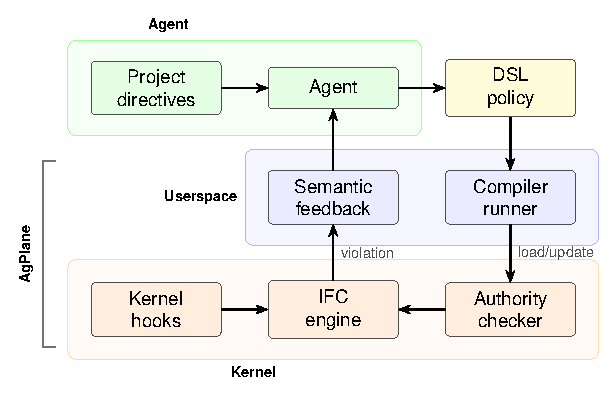
\includegraphics[width=\columnwidth]{figures/architecture.pdf}
\caption{\sys{} architecture: policy generation, compilation, kernel
enforcement, and feedback loop.}
\Description{Three-layer diagram: agent (directives, LLM), userspace
(compiler, feedback), kernel (hooks, IFC engine, authority checker).}
\label{fig:architecture}
\end{figure}

\subsection{Policy DSL}
\label{sec:dsl}

The DSL mediates between AI agent intent and enforceable system actions.
A policy contains \emph{sources} that introduce labels,
\emph{rules} that match labeled events at sinks, and optional
\emph{gates} that express cross-event ordering constraints. The
DSL restricts expressiveness to source/sink/gate patterns that compile
to fixed-size rodata, enabling bounded verification cost and
agent-authorability.

Sources bind labels to system objects: an \texttt{exec} source labels
processes that execute a matching binary; a \texttt{file} source labels
matching paths; a network source labels matching endpoints. Rules bind an
effect (\texttt{notify}, \texttt{block}, or \texttt{kill}) to an
operation (\texttt{exec}, \texttt{read}, \texttt{write},
\texttt{unlink}, or \texttt{connect}). Conditions express common agent
workflow constraints: a target allow-list, a lineage gate, or a temporal
\texttt{after~...~since~...} ordering gate.

\begin{figure}[t]
\begin{verbatim}
source AGENT = exec "claude"
source SECRET = file "**/.env"

# Per-event: from CoplayDev/unity-mcp
rule no-push-main:
  kill exec "git" "push" "main" if AGENT
  because "Do not push to main; open a PR instead."

# Cross-event: from chenhg5/cc-connect
rule tests-before-commit:
  block exec "git" "commit"
    if AGENT unless after exec "go" since write "**/*.go"
  because "Run `go test ./...` before committing."
\end{verbatim}
\caption{Two \sys{} rules drawn from real projects. The first is a
per-event rule; the second is a cross-event rule that requires temporal
state.}
\Description{Code listing of two \sys{} rules from real projects.}
\label{fig:policy-example}
\end{figure}

Figure~\ref{fig:policy-example} illustrates the two main rule shapes. The
first is per-event: if the agent process pushes to \texttt{main}, the
event matches immediately. The second is cross-event: committing is
compliant only if the required test command ran after the most recent
source write. This distinction motivates the DSL's two predicate
classes: per-event matches and cross-event gates.

The DSL is intentionally narrower than a general mandatory access-control
language. It targets the policy shapes that recur in agent instruction
files: prohibit a command, restrict writes to a scope, block a sink after
a sensitive read, require a validation step before a release action, and
route sensitive data through an approved tool. The compiler lowers these
patterns into fixed-size kernel tables; policy authors need not reason
about BPF maps, verifier constraints, or binary layout.

\subsection{Labeled Information-Flow Model}
\label{sec:ifc}

\sys{} represents policy state as labels on OS objects. Processes, files,
and network endpoints each carry a 64-bit label mask, enabling
cross-boundary flow policies (e.g., ``data read from \texttt{.env} must
not reach a network endpoint''). A source declaration adds labels when an
object matches the source pattern. Let $L(x)$ denote
the label mask of object $x$. Labels propagate through observed
system-level edges:

\begin{itemize}
\item \textbf{fork}$(p \to c)$: $L(c) := L(c) \cup L(p)$.
\item \textbf{exec}$(p, f)$: $L(p) := L(p) \cup L(f) \cup S(f)$, where
$S(f)$ is the set of source labels matching $f$.
\item \textbf{read}$(p, f)$: $L(p) := L(p) \cup L(f)$.
\item \textbf{write}$(p, f)$: $L(f) := L(f) \cup L(p)$.
\item \textbf{connect}$(p, e)$: $L(e) := L(e) \cup L(p)$.
\end{itemize}

These transfer functions maintain a key invariant: if an object carries
label $\ell$, then information from a source tagged with $\ell$ has
reached that object through observed execution edges. Rules check whether
an event's subject or target carries required labels, carries forbidden
labels, or satisfies a temporal gate.

The model operates at object granularity rather than byte granularity,
trading precision for low-overhead whole-session coverage. This is a
deliberate fit for AI agent harnesses: repository instructions refer to
commands, files, directories, endpoints, and workflow steps, not
individual bytes. Object-level labels capture cross-event compliance
patterns that tool-call filters miss, without incurring the complexity of
byte-level taint tracking~\cite{kemerlis2012libdft}.

Labels are monotonic: propagation adds labels but never removes them.
Once an object carries a label, every subsequent consumer inherits it.
This ensures that cross-event constraints remain checkable for the
entire session without requiring explicit label cleanup.

\subsection{Layered Policy Authority}
\label{sec:authority}

Agents must adapt policy at runtime: a sub-agent spawned for a narrow
sub-task should operate under tighter constraints, and the current task
may require an exception to a standing rule; but adaptation must never
weaken platform or project constraints.

\sys{} organizes policy as a layered authority stack:
platform/operator, project-maintainer, and agent/session. Policy
evolution is \emph{monotonically tightening}: each layer may add rules,
specialize targets, introduce labels, or narrow scope, but no layer may
delete, rewrite, or weaken rules from a higher-authority
layer. When an agent forks a sub-agent, the child inherits the parent's
label set and effective rules; the sub-agent may add further restrictions
but cannot shed inherited constraints.

Higher-authority rules that admit exceptions use the same gate mechanism
as cross-event rules: the rule names an explicit action the agent must
perform to satisfy the condition. For example, a project rule ``do not
force-push unless necessary'' can require the agent to write a
declaration file (e.g., \texttt{.actplane/force-push-necessary}) before
the push is allowed. The agent satisfies the gate by creating the file, which the IFC
engine tracks like any other label-propagating event. Higher-authority policy can further constrain
which processes may write the declaration file, keeping exception paths
under platform or project authority.

The prototype resolves the initial authority stack at compile or load
time. Each compiled policy blob carries an authority tag (platform,
project, or agent); the kernel authority checker accepts a new blob only
if it is additive with respect to all higher-tagged blobs already
installed. Concretely, the checker rejects any update that deletes an
existing rule, widens a target pattern, or introduces a gate that clears
a label from a higher authority level. Runtime policy additions
(sub-agent restrictions, task-specific rules) are loaded as additive
overlays through a userspace ring buffer; the kernel merges them with the
existing rule tables after the authority check passes. The kernel does
not parse configuration or resolve project context on the event path;
agents supply context and policy structure, while the OS engine enforces
the compiled result uniformly across tools and subprocesses.

\section{Implementation}
\label{sec:implementation}

\sys{} consists of a Rust compiler/runner (~3.2\,K\,LoC) and an eBPF
enforcement engine (~1.8\,K\,LoC of BPF C). The compiler parses the DSL,
allocates label bits, lowers Boolean label expressions and path/network
patterns, and emits a fixed-size \texttt{\#[repr(C)]} configuration blob
consumed directly by the eBPF loader. Human-readable rule names and
reasons stay in userspace metadata; the kernel receives only compact rule
tables and emits rule identifiers when events match.

The eBPF engine attaches to process, file, and network hooks via BPF-LSM
(pre-operation enforcement) and tracepoints (observation and
post-operation termination). It maintains label state in per-object BPF
maps, applies the transfer functions from \S\ref{sec:design}, and
evaluates the compiled rules on each observed event. Userspace does not
re-detect violations: it loads the policy, starts the target process, and
formats kernel-reported matches into semantic feedback.

The runner (\texttt{actplane run -- <cmd>}) discovers the project policy
file, compiles and loads it before the target starts, seeds the target
process tree with the agent label, and records kernel matches in a
feedback file. Compatible agent hooks relay this feedback into the model's
next turn. The runner is intentionally thin: the policy decision stays in
the kernel, while the runner only connects policy, execution, and
agent-facing diagnostics.
